\documentclass[journal,twoside,print]{ieeecolor}
\usepackage{generic}
\usepackage{review_layout}
\usepackage[T1]{fontenc}
\usepackage[utf8]{inputenc}
\usepackage{cite,amsmath,amssymb,graphicx,url,booktabs,array,needspace,balance}
\def\journalname{}
\markboth{}{CHAN: Re-evaluating Multimodal LLMs for Influenza Forecasting}
\begin{document}
\title{Re-evaluating Multimodal LLMs for Influenza Forecasting: A 28-Model Empirical Benchmark}
\author{\mbox{CHAN~Sing~Yeung}\thanks{CHAN Sing Yeung is with the Department of Electrical Engineering, City University of Hong Kong, Hong Kong (e-mail: sychan552-c@my.cityu.edu.hk).}}
\maketitle
\begin{abstract}
Average forecast error can conceal differences in epidemic peak timing, peak magnitude and model size. We evaluate these trade-offs in a reproducibility study of multimodal influenza forecasting. The retained benchmark contains 28 implementations evaluated on a 966-week national influenza series with seven numerical channels, four forecast lengths and three seeds. Accuracy and peak analyses cover all implementations, whereas parameter analysis and paired testing cover explicitly defined subsets of 11 and 17 models. MIFlu has the lowest observed mean squared error at 1.5574, followed by PatchTST at 1.6621 and NLinear at 1.8716. NLinear has lower mean peak-intensity error than MIFlu, but higher mean peak-timing error. Both satisfy a joint timing-and-height screen in four of 16 aggregated cells; PatchTST satisfies none. In the parameter subset, PatchTST uses approximately 211 times as many parameters as NLinear for 11.2\% lower observed mean squared error. Recomputed Holm adjustments reject none of 136 comparisons, a result limited by the documented test resolution rather than evidence of equivalence. Eleven frozen language encoders under a linear readout underperform a decision-tree baseline. These findings support reporting peak timing and magnitude alongside average accuracy and explicitly distinguishing parameter count from measured computational cost. The results remain exploratory and do not establish prospective public-health utility or a causal benefit from multimodal inputs.
\end{abstract}
\begin{IEEEkeywords}
Epidemic forecasting, influenza, large language models, peak prediction, reproducibility, time series
\end{IEEEkeywords}
\Needspace{5\baselineskip}
\section{Introduction}
Influenza forecasts can support preparedness, but a model that minimises average error need not minimise the error of a disease peak. Peak timing affects when resources are needed, while peak magnitude affects the scale of preparation. Kramer and Shaman evaluate these endpoints separately in influenza forecasting \cite{r2}. An empirical model comparison should therefore state which outcome defines a useful forecast instead of treating one aggregate accuracy ranking as a deployment decision.

Large language models offer several ways to combine numerical sequences and textual information. MIFlu applies a multimodal design to influenza prediction \cite{r1}, while Time-LLM, CALF and TimeCMA use distinct reprogramming or alignment mechanisms \cite{r6,r7,r8}. At the same time, strong linear forecasting results and language-model removal studies challenge the assumption that additional architectural complexity necessarily improves prediction \cite{r4,r13}. A later preprint reports conditional benefits under broader cross-dataset settings \cite{r14}. These findings motivate a task-specific assessment with explicit implementation and evaluation boundaries.

We study how model choice changes across average accuracy, peak errors, parameter count and statistical evidence. Our contributions are an influenza-specific comparison of 28 retained implementations, a timing--height analysis of their peak forecasts, and an audit of the parameter and paired-test subsets. We also distinguish an independent reproduction comparison from the broader benchmark and examine a fixed-weight text-input pathway. The study evaluates existing implementations; it does not introduce a new forecasting architecture or establish a universal conclusion about language models.

\Needspace{5\baselineskip}
\section{Related Work}
PatchTST and iTransformer provide transformer baselines with different tokenisations of time-series information \cite{r3,r5}. Zeng et al. show that simple linear baselines can challenge transformer forecasting methods \cite{r4}. Tan et al. examine whether language-model components are necessary in time-series systems \cite{r13}. Our evaluation follows this comparative motivation, but its evidence is restricted to one influenza dataset and the retained implementations.

The label LLM-based encompasses different mechanisms. Time-LLM combines a frozen backbone with learned reprogramming and prompt information \cite{r6}. CALF and TimeCMA use cross-modal alignment designs \cite{r7,r8}. A frozen encoder followed by a linear readout is a narrower experimental configuration and cannot stand in for prompting, generation or fine-tuning. Chronos, TimesFM, Moirai and Lag-Llama instead learn from numerical time series \cite{r9,r10,r11,r12}. Their absence from the present comparison limits any claim about modern time-series foundation models.

Forecast evaluation also depends on the target scale, the sampling units and the uncertainty being estimated. Hyndman and Koehler discuss the consequences of forecast-error measurement \cite{r21}, while Bouthillier et al. distinguish repeated-run variability from broader benchmark variation \cite{r19}. Demšar describes comparison procedures across multiple models \cite{r20}. These considerations are important here because multiple seeds and forecast lengths reuse the same underlying national series; they are not independent epidemics.

\Needspace{5\baselineskip}
\section{Data and Evaluation Protocol}
\Needspace{3\baselineskip}
\subsection{Dataset and chronological separation}
The evaluation uses a US national influenza series distributed with the project reproduction materials. It contains 966 ordered weekly observations and seven numerical channels. The chronological split contains 676 training, 97 validation and 193 test rows. Scaling is fitted on the training block and applied without refitting to later observations. Checkpoints are selected by validation performance. This separation avoids using the final test block to estimate preprocessing constants or select the reported model \cite{r22}.

Two local versions of the data agree numerically across their seven matched channels. Their byte identity with a pinned, independently obtained author revision is not established. The available date labels are synthetic, so we use relative week indices and do not assign the detected peaks to independently verified epidemiological seasons. This distinction affects the external interpretation of peak results.

\Needspace{3\baselineskip}
\subsection{Reproduction and benchmark estimands}
The reproduction comparison uses ten seeds, 2021--2030, to compare local MIFlu estimates with the tabulated reference in Moon et al. \cite{r1}. The retained benchmark uses seeds 42, 43 and 44 to compare implementations under its declared evaluation contract. These estimates serve different questions and are reported separately. Table I summarises the analysis populations. Three seeds reflect the available compute budget; they are not a universal forecasting convention. PatchTST and iTransformer provide five-run robustness evidence in their respective evaluations \cite{r3,r5}.

The history length is 104 weeks and forecast lengths are 24, 36, 48 and 60 weeks. The corresponding test sets contain 170, 158, 146 and 134 available forecast windows. The historical comparison retains complete batches of 16, yielding 160, 144, 144 and 128 scored windows. Its tables refer to this shared cropped-window contract. Removing a tail of observations can change results, so a full-window sensitivity analysis remains necessary. An ongoing ten-seed expansion is excluded from the scientific tables because stored scoring windows have not yet been harmonised across its implementations.

\begin{table}[!t]
\caption{Separate evaluation populations and run sets}
\label{tab:protocol}
\centering
\footnotesize
\setlength{\tabcolsep}{3pt}
\begin{tabular}{@{}>{\raggedright\arraybackslash}p{0.2552\columnwidth}>{\raggedright\arraybackslash}p{0.2955\columnwidth}>{\centering\arraybackslash}p{0.3493\columnwidth}@{}}
\toprule
Analysis & Runs or models & Evaluation \\
\midrule
Reproduction & MIFlu; 10 seeds & Reference-table comparison \\
Accuracy and peaks & 28 models; 3 seeds & 4 lengths; 16 peak cells/model \\
Parameters & 11 models & Exported size and MSE \\
Paired comparisons & 17 models & 136 pairs; 12 contributions/pair \\
\bottomrule
\end{tabular}
\par\smallskip\begin{minipage}{\columnwidth}\footnotesize The roster contains 13 conventional models, four LLM-based models and 11 frozen encoders. Each analysis uses its stated denominator.\end{minipage}
\end{table}
\Needspace{3\baselineskip}
\subsection{Model roster and implementation scope}
The 28 retained arms comprise 13 conventional models, four LLM-based implementations and 11 frozen language encoders. The conventional group contains five classical machine-learning models, five neural models, two transformers and one linear model. The LLM-based group contains MIFlu, TimeCMA, Qwen-Time and CALF. The frozen-encoder group uses a fixed encoder and a trained linear readout.

Accuracy and peak analyses cover all 28 retained arms. The parameter export covers 11 models, and the archived paired-test family covers the 17 non-encoder models, including MIFlu. DLinear is outside the historical retained roster and paired family. Its exclusion limits baseline coverage and requires a sensitivity comparison. Model names identify the project implementations; their ranking does not certify exact implementation fidelity to every cited method. In particular, preprocessing, checkpoint selection and training settings must be matched before attributing a discrepancy to a single implementation change.

\Needspace{5\baselineskip}
\section{Evaluation Methods}
\Needspace{3\baselineskip}
\subsection{Average forecast error}
Mean squared error and mean absolute error are computed in the standardised seven-channel space and aggregated over the scored predictions. The reported benchmark mean then averages the four forecast lengths. Standardising each channel avoids allowing one numerical scale to dominate the aggregate, but the resulting loss is dimensionless. It is not a patient-count series and cannot be inverted using one scaler. Peak endpoints are therefore evaluated on a specific channel, ILITOTAL, after its own inverse transform \cite{r21}.

\Needspace{3\baselineskip}
\subsection{Peak timing and intensity}
For a matched observed and predicted peak, peak-timing error is the absolute difference between their week indices. Peak-intensity error is the absolute height difference divided by the observed peak height, expressed as a percentage. We use the separate one-week timing and 25\% intensity tolerances described by Kramer and Shaman \cite{r2}. Our joint screen requires both tolerances to hold for the aggregated mean errors in a model--forecast-length--lead cell.

The detector uses a prominence of 0.15 times the series range, a minimum distance of 15 weeks and matching within eight weeks. These detector settings and the conjunction applied to aggregated means are project choices. Four forecast lengths and four leads produce 16 cells per model. A count such as 4/16 is therefore neither a seasonal success probability nor a calibrated probability of a future surge. Peak detection and matching are retrospective and can use observations unavailable at the original forecast issue time.

\Needspace{3\baselineskip}
\subsection{Parameter frontier}
We compare mean squared error with exported parameter count for the 11 models with available values. A model is dominated if another model has no greater error and no more parameters, with at least one strict improvement. The remaining models form the frontier of this measured subset. Missing parameter counts are not treated as zero. Parameter count measures model size; latency, peak memory, energy consumption and monetary cost require separate measurements. iTransformer illustrates evaluation of prediction error alongside measured computational resources \cite{r5}.

\Needspace{3\baselineskip}
\subsection{Paired comparisons and multiplicity}
The archived tests contain 136 pairwise comparisons among 17 models, using 12 matched forecast-length--seed contributions per pair. We retain the exported raw p-values and recompute Holm adjustments by sorting the p-values, multiplying by the remaining family size, and taking a forward cumulative maximum \cite{r20}. The exported adjusted-p column is not used because its cumulative operation was incorrect. Rounded exports are also mapped back to their documented 1/4096 enumeration grid; the difference does not affect the displayed four-decimal adjusted values.

For the documented two-sided exact sign-flip test with 12 contributions, the smallest raw p-value is 2/4096. Multiplication by the first Holm factor of 136 gives 0.06640625, above the 0.05 familywise threshold. The first rejection is therefore unattainable at that resolution. This arithmetic limit is separate from the exchangeability assumptions of the raw test. Shared observations and overlapping forecast lengths also restrict interpretation of the contributions as independent sampling units. We treat the comparisons as exploratory and do not infer equivalence from non-rejection \cite{r25}.

\Needspace{3\baselineskip}
\subsection{Text-pathway functional checks}
In the evaluated author-faithful MIFlu pathway, numerical time tokens precede text tokens in a causal-attention sequence, and the forecast head reads only time-token positions. Causal masking prevents those positions from attending to subsequent text positions \cite{r24}. We inspect this pathway and use three archived CPU checks that control inputs, model initialisation and evaluation conditions when changing text or comparing matched full/no-text outputs. These checks concern a fixed-weight forward computation. They do not test equality of independent training trajectories or isolate the contribution of pretrained weights or adaptation parameters.

\Needspace{5\baselineskip}
\section{Results}
\Needspace{3\baselineskip}
\subsection{Independent reproduction comparison}
Table II reports the reproduction comparison. The mean squared error is 1.4995 compared with the reference value 1.4355, a 4.5\% increase. Error is lower at forecast lengths 24 and 36, but higher at 48 and 60. Mean absolute error is 0.8043 compared with 0.7452, a 7.9\% increase; only the 36-week result is lower than its reference. The two error measures therefore do not have the same horizon-wise pattern.

\begin{table}[!t]
\caption{MIFlu reproduction under its separate ten-seed protocol}
\label{tab:reproduction}
\centering
\footnotesize
\setlength{\tabcolsep}{3pt}
\begin{tabular}{@{}>{\raggedright\arraybackslash}p{0.129\columnwidth}>{\raggedright\arraybackslash}p{0.2687\columnwidth}>{\centering\arraybackslash}p{0.1693\columnwidth}>{\centering\arraybackslash}p{0.1639\columnwidth}>{\centering\arraybackslash}p{0.1693\columnwidth}@{}}
\toprule
Length & Our MSE $\pm$ SD & Reference MSE & Our MAE & Reference MAE \\
\midrule
L=24 & 1.3045 $\pm$ 0.0883 & 1.5420 & 0.7482 & 0.7260 \\
L=36 & 1.3561 $\pm$ 0.1603 & 1.4220 & 0.7712 & 0.7790 \\
L=48 & 1.6543 $\pm$ 0.1064 & 1.4140 & 0.8381 & 0.7570 \\
L=60 & 1.6829 $\pm$ 0.2109 & 1.3640 & 0.8596 & 0.7190 \\
4-horizon mean & 1.4995 & 1.4355 & 0.8043 & 0.7452 \\
\bottomrule
\end{tabular}
\par\smallskip\begin{minipage}{\columnwidth}\footnotesize SD is reconstructed from the archived score record. Original run predictions are unavailable for independent rescoring. The four-length row reports the aggregate comparison.\end{minipage}
\end{table}
The table is an arithmetic comparison with the published reference, rather than evidence of superiority or a completed exact replication. The reported standard deviations are reconstructed from the archived, code-transcribed ten-seed score record; saved predictions and logs for those reproduction runs are not available for independent rescoring. Protocol and upstream-version uncertainty prevent assigning the observed gap to one causal change.

\Needspace{3\baselineskip}
\subsection{Average-error ranking}
MIFlu has the lowest observed benchmark mean squared error, 1.5574. PatchTST and NLinear follow at 1.6621 and 1.8716, with corresponding mean absolute errors of 0.8786 and 0.9183 compared with MIFlu's 0.8199. These are means under the three benchmark seeds, not the ten-seed reproduction estimates. Table III reports all retained implementations. The result does not by itself establish that multimodal inputs caused MIFlu's ranking.

\begin{table}[!t]
\caption{Average errors of the 28 retained implementations}
\label{tab:accuracy}
\centering
\footnotesize
\setlength{\tabcolsep}{3pt}
\begin{tabular}{@{}>{\raggedright\arraybackslash}p{0.1209\columnwidth}>{\raggedright\arraybackslash}p{0.3842\columnwidth}>{\centering\arraybackslash}p{0.1988\columnwidth}>{\centering\arraybackslash}p{0.1961\columnwidth}@{}}
\toprule
Rank & Implementation & \shortstack{Mean\\MSE} & \shortstack{Mean\\MAE} \\
\midrule
1 & MIFlu & 1.5574 & 0.8199 \\
2 & PatchTST & 1.6621 & 0.8786 \\
3 & NLinear & 1.8716 & 0.9183 \\
4 & DNN & 2.1415 & 1.0057 \\
5 & TimeCMA & 2.6081 & 1.0676 \\
6 & Gradient Boosting & 3.6645 & 1.2521 \\
7 & KNN & 3.7854 & 1.3293 \\
8 & Random Forest & 3.8901 & 1.2779 \\
9 & iTransformer & 3.9945 & 1.3476 \\
10 & Decision Tree & 4.3198 & 1.3798 \\
11 & Hunyuan-1.8B & 4.7374 & 1.4755 \\
12 & Hunyuan-7B & 4.7596 & 1.4685 \\
13 & DeepSeek-R1-Qwen-1.5B & 4.7866 & 1.5002 \\
14 & DeepSeek-R1-Llama-8B & 4.8250 & 1.4786 \\
15 & GRU & 4.8870 & 1.5174 \\
16 & DeepSeek-R1-32B & 4.9372 & 1.4935 \\
17 & LSTM & 5.0088 & 1.5303 \\
18 & DeepSeek-R1-Qwen-14B & 5.0166 & 1.5019 \\
19 & DeepSeek-R1-Qwen-7B & 5.0308 & 1.5133 \\
20 & RNN & 5.0674 & 1.5634 \\
21 & ContextPilot-8B & 5.0843 & 1.5255 \\
22 & Hunyuan-4B & 5.1317 & 1.5450 \\
23 & ContextPilot-14B & 5.1949 & 1.5407 \\
24 & Qwen2.5-1.5B & 5.2049 & 1.5725 \\
25 & Qwen-Time & 5.2557 & 1.5794 \\
26 & SVR & 5.3388 & 1.4986 \\
27 & CALF & 5.5785 & 1.6190 \\
28 & CNN & 5.6155 & 1.6720 \\
\bottomrule
\end{tabular}
\par\smallskip\begin{minipage}{\columnwidth}\footnotesize Three benchmark seeds, four forecast lengths and the declared cropped-window contract. Names label project implementations; method fidelity is not established by the ranking.\end{minipage}
\end{table}
\Needspace{3\baselineskip}
\subsection{Peak timing and height}
Table IV summarises the peak endpoints. NLinear has lower mean peak-intensity error than MIFlu, 9.477\% versus 26.846\%, but higher mean peak-timing error, 1.677 versus 1.128 weeks. Both pass the joint screen in 4/16 aggregated cells, while PatchTST passes 0/16. Equal pass counts conceal different locations: NLinear passes the first lead at all four forecast lengths; MIFlu passes the first lead at lengths 24, 36 and 60 and the second lead at length 48.

\begin{table}[!t]
\caption{Mean peak errors and the joint aggregated-cell screen}
\label{tab:peaks}
\centering
\footnotesize
\setlength{\tabcolsep}{3pt}
\begin{tabular}{@{}>{\raggedright\arraybackslash}p{0.2767\columnwidth}>{\raggedright\arraybackslash}p{0.2096\columnwidth}>{\centering\arraybackslash}p{0.2096\columnwidth}>{\centering\arraybackslash}p{0.2042\columnwidth}@{}}
\toprule
Model & PTE (weeks) & PIE (\%) & Joint passes \\
\midrule
MIFlu & 1.128 & 26.846 & 4/16 \\
PatchTST & 1.240 & 32.755 & 0/16 \\
NLinear & 1.677 & 9.477 & 4/16 \\
\bottomrule
\end{tabular}
\par\smallskip\begin{minipage}{\columnwidth}\footnotesize The denominator is four forecast lengths times four leads. A pass requires mean PTE at most one week and mean PIE at most 25\% in the same cell; it is not a seasonal success probability.\end{minipage}
\end{table}
Among the leading three models, the MSE ordering is MIFlu, PatchTST, NLinear, whereas the peak-intensity ordering is NLinear, MIFlu, PatchTST. The order is inverted at both ends. Fig. 1 shows the full comparison. Across all 28 models, the Spearman association between MSE and peak-intensity error remains positive at approximately 0.736, and the association with joint-pass count is approximately -0.429. A local ordering difference therefore coexists with an overall association; it does not demonstrate statistical independence or universal peak-skill decoupling.

\begin{figure}[!t]
\centering
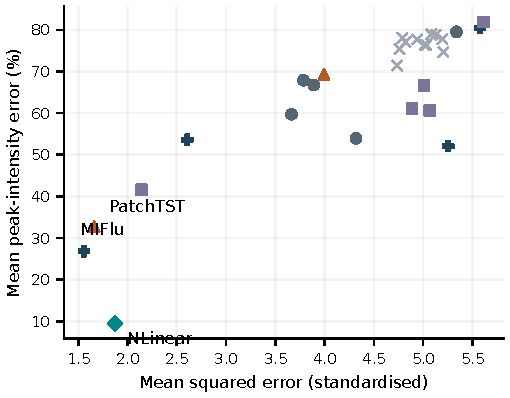
\includegraphics[width=\columnwidth]{figures/peak_scatter.pdf}
\caption{Mean MSE and mean peak-intensity error across the 28 retained implementations. Each point is a model aggregate, not an independent epidemic. The leading models differ locally despite a positive overall rank association.}
\label{fig:peak_scatter}
\end{figure}
\Needspace{3\baselineskip}
\subsection{Parameter trade-off}
Fig. 2 shows two frontier members in the 11-model parameter subset: NLinear with 2,520 parameters and PatchTST with 531,878. PatchTST uses approximately 211.1 times as many parameters for 11.2\% lower observed MSE. Neither dominates the other on both axes. MIFlu and the frozen encoders are absent from this subset, so the result is not a frontier over all 28 models.

\begin{figure}[!t]
\centering
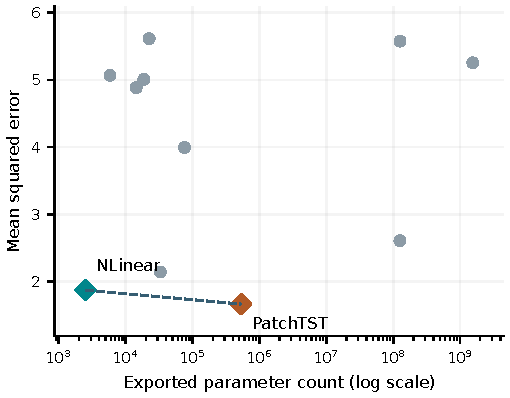
\includegraphics[width=\columnwidth]{figures/pareto.pdf}
\caption{Size--error frontier for the 11 models with parameter exports. The dashed segment joins the two nondominated choices in this subset. Parameter count is a size proxy; MIFlu and frozen encoders have no exported value and are excluded.}
\label{fig:pareto}
\end{figure}
The fitted slope of MSE against log10 parameter count is approximately +0.1171 and the coefficient of determination is 0.0223. This cross-model association explains little of the observed error variation within the measured subset. It does not isolate the causal effect of model capacity: architecture, optimisation, tuning and training regime also vary. Likewise, the parameter ratio is not a measured runtime or energy ratio.

\Needspace{3\baselineskip}
\subsection{Corrected statistical evidence}
Table V gives selected paired comparisons. Before adjustment, 128 of 136 raw p-values are below 0.05. After correct Holm adjustment, none is below 0.05. The minimum adjusted value is approximately 0.0664, consistent with the resolution bound. The adjusted NLinear--PatchTST value is 0.1172. PatchTST nevertheless has lower error in 10 of the 12 matched contributions and an 11.2\% lower observed aggregate MSE. The absence of a familywise rejection neither removes that descriptive difference nor establishes practical equivalence.

\begin{table}[!t]
\caption{Selected comparisons with recomputed Holm adjustment}
\label{tab:paired}
\centering
\footnotesize
\setlength{\tabcolsep}{3pt}
\begin{tabular}{@{}>{\raggedright\arraybackslash}p{0.2713\columnwidth}>{\raggedright\arraybackslash}p{0.2687\columnwidth}>{\centering\arraybackslash}p{0.1827\columnwidth}>{\centering\arraybackslash}p{0.1773\columnwidth}@{}}
\toprule
Model A & Model B & Raw p & Adjusted p \\
\midrule
NLinear & PatchTST & 0.005859 & 0.1172 \\
Gradient Boosting & RNN & 0.000488 & 0.0664 \\
KNN & NLinear & 0.000488 & 0.0664 \\
KNN & MIFlu & 0.000488 & 0.0664 \\
KNN & LSTM & 0.000488 & 0.0664 \\
iTransformer & TimeCMA & 0.000488 & 0.0664 \\
iTransformer & SVR & 0.000488 & 0.0664 \\
\bottomrule
\end{tabular}
\par\smallskip\begin{minipage}{\columnwidth}\footnotesize Family: 17 non-encoder models including MIFlu, excluding DLinear and frozen encoders. There are 136 pairs and 12 matched contributions per pair. Raw p-values are rounded exports; adjusted values shown at four decimals.\end{minipage}
\end{table}
\Needspace{3\baselineskip}
\subsection{Frozen language features and text dependence}
All 11 frozen encoders under the shared linear readout have MSE between 4.7374 and 5.2049, approximately 3.04--3.34 times MIFlu's value. Each exceeds the decision-tree baseline of 4.3198 and passes 0/16 joint cells. The failure is specific to this frozen-feature/readout protocol. It does not evaluate generation, prompting, end-to-end adaptation or numerical time-series foundation models.

The three fixed-weight CPU functional checks pass without skips. They support output invariance to the tested text changes and equality of the matched full/no-text forward outputs in the inspected pathway. The result concerns inference-time dependence under controlled conditions. It does not establish that language pretraining or adaptation is unnecessary during training. No predictive effect is assigned to network depth or adaptation removal because the per-variant training results have not yet been aggregated and verified.

\Needspace{5\baselineskip}
\section{Discussion}
\Needspace{3\baselineskip}
\subsection{Implications for model selection}
The main empirical distinction is between average-error preference and peak-error preference. MIFlu leads the observed aggregate MSE ranking, while NLinear offers lower mean peak-height error at low parameter count. Its higher mean timing error prevents a claim of overall peak superiority. Even the same joint-pass count can represent different lead-dependent strengths. An application must therefore specify whether timing, magnitude or another forecast outcome matters before choosing a model.

The findings do not support equating a lower standardised loss with demonstrated public-health benefit. A decision-oriented comparison would define the cost of missed peaks and false alarms on validation data, then evaluate the selected rule at held-out origins. Such a study would require a verified calendar, prospective issue-time information and outcome-specific uncertainty. The present retrospective screen is useful for comparing errors but does not establish a deployment threshold.

\Needspace{3\baselineskip}
\subsection{Interpretation of multimodal contribution}
The functional check and model ranking address different questions. A multimodal architecture can perform well even when one inspected text pathway is masked at inference. The observed score does not isolate which learned components are responsible. Conversely, poor performance from frozen language features does not establish that all LLM-based forecasting is ineffective. Matched controls for pretraining, readout, alignment and adaptation are needed to separate these explanations \cite{r6,r13}.

\Needspace{3\baselineskip}
\subsection{Statistical and computational interpretation}
The Holm resolution bound shows why adding a correction to a coarse exact test does not automatically produce an informative model-selection procedure. Additional seeds can improve precision for repeated training, but they do not create independent epidemics \cite{r19}. Future inference should preserve the temporal and cross-model dependence of forecasts and report effect estimates alongside uncertainty. Equivalence would require a justified margin and an appropriate design \cite{r25}.

The parameter frontier is similarly conditional. NLinear and PatchTST describe two size--error choices within an incomplete resource export. A full efficiency comparison should measure comparable inference and training costs under stated hardware, batch size and forecast length \cite{r5}. The present results do not establish latency, memory or energy savings.

\Needspace{5\baselineskip}
\section{Limitations}
The evaluation uses one national series and one chronological split. It cannot establish regional transfer or prospective utility. Synthetic calendar labels prevent verified season-specific interpretation, and retrospective peak matching may use future observations. Full-window sensitivity and rolling-origin evaluation are needed before interpreting a retained-window result as stable across time \cite{r23}.

Implementation fidelity and baseline coverage remain incomplete. The exact upstream data and code revision for the reference reproduction is unresolved, DLinear is absent from the retained historical roster, and modern numerical foundation models are not included. Frozen-encoder results cannot substitute for those controls. Missing parameter exports also prevent a resource frontier for the entire roster.

The ongoing expansion is not included in the reported rankings. Its stored metrics currently mix cropped MIFlu windows and full windows for other models; complete seven-channel MIFlu predictions are needed for a common rescore. The expansion protocol was not frozen before execution and is not treated as prospectively registered confirmation. More completed jobs alone would not resolve these evaluation differences.

The paired analysis reuses exported raw p-values rather than reconstructing every raw paired prediction comparison. Its matched cells are dependent, its test has coarse resolution and the source effect measure uses pooled model variability rather than variability of paired differences. We therefore do not present source confidence intervals or effect-size values as validated independent-sample inference. Per-variant predictive ablation effects and calibrated predictive uncertainty also remain unestablished.

\Needspace{5\baselineskip}
\section{Conclusion}
Across the retained influenza implementations, the model with the lowest average MSE does not have the lowest peak-height error. MIFlu, NLinear and PatchTST illustrate distinct accuracy, timing, magnitude and parameter trade-offs, while correct multiplicity adjustment yields no familywise rejection at the documented test resolution. The frozen-feature negative result and the fixed-weight text-pathway check apply to specific implementations and do not establish a universal causal claim about language models. The practical contribution is an explicit evaluation contract and a bounded comparison of forecast outcomes. Harmonised scoring, stronger controls and validation across origins and regions are required before making a deployment claim.

\Needspace{5\baselineskip}
\section{Data and Code Availability}
The analysis is reproducible from the archived benchmark tables and accompanying scoring code. A public archive for this exact experimental revision and a pinned upstream reference implementation have not yet been established. The complete comparison should be reassessed when harmonised prediction-level evidence becomes available.

\balance\begin{thebibliography}{99}
\bibitem{r2} Sarah C. Kramer and Jeffrey Shaman, ``Development and validation of influenza forecasting for 64 temperate and tropical countries,'' PLOS Computational Biology 15(2), e1006742, 2019. \url{https://doi.org/10.1371/journal.pcbi.1006742}
\bibitem{r1} Jaeuk Moon, Jonghwa Shim, Eunbeen Kim and Eenjun Hwang, ``MIFlu: Large Language Model-Based Multimodal Influenza Forecasting Scheme,'' IEEE JBHI 29(10), 7790-7801, 2025. \url{https://doi.org/10.1109/JBHI.2025.3561214}
\bibitem{r6} Ming Jin et al., ``Time-LLM: Time Series Forecasting by Reprogramming Large Language Models,'' ICLR, 2024. \url{https://arxiv.org/abs/2310.01728}
\bibitem{r7} Peiyuan Liu et al., ``CALF: Aligning LLMs for Time Series Forecasting via Cross-modal Fine-Tuning,'' arXiv:2403.07300, 2024. \url{https://arxiv.org/abs/2403.07300}
\bibitem{r8} Chenxi Liu et al., ``TimeCMA: Towards LLM-Empowered Multivariate Time Series Forecasting via Cross-Modality Alignment,'' AAAI, 2025. \url{https://arxiv.org/abs/2406.01638}
\bibitem{r4} Ailing Zeng, Muxi Chen, Lei Zhang and Qiang Xu, ``Are Transformers Effective for Time Series Forecasting?,'' AAAI, 2023. \url{https://arxiv.org/abs/2205.13504}
\bibitem{r13} Mingtian Tan, Mike A. Merrill, Vinayak Gupta, Tim Althoff and Thomas Hartvigsen, ``Are Language Models Actually Useful for Time Series Forecasting?,'' NeurIPS 37, 2024. \url{https://arxiv.org/abs/2406.16964}
\bibitem{r14} Xin Qiu et al., ``Rethinking the Role of LLMs in Time Series Forecasting,'' arXiv:2602.14744 v1, preprint, 2026. \url{https://arxiv.org/abs/2602.14744}
\bibitem{r3} Yuqi Nie, Nam H. Nguyen, Phanwadee Sinthong and Jayant Kalagnanam, ``A Time Series is Worth 64 Words: Long-term Forecasting with Transformers,'' ICLR, 2023. \url{https://arxiv.org/abs/2211.14730}
\bibitem{r5} Yong Liu et al., ``iTransformer: Inverted Transformers Are Effective for Time Series Forecasting,'' ICLR, 2024. \url{https://arxiv.org/abs/2310.06625}
\bibitem{r9} Abdul Fatir Ansari et al., ``Chronos: Learning the Language of Time Series,'' Transactions on Machine Learning Research, 2024. \url{https://arxiv.org/abs/2403.07815}
\bibitem{r10} Abhimanyu Das, Weihao Kong, Rajat Sen and Yichen Zhou, ``A decoder-only foundation model for time-series forecasting,'' ICML, PMLR 235, 10148-10167, 2024. \url{https://proceedings.mlr.press/v235/das24c.html}
\bibitem{r11} Gerald Woo et al., ``Unified Training of Universal Time Series Forecasting Transformers,'' ICML, PMLR 235, 53140-53164, 2024. \url{https://proceedings.mlr.press/v235/woo24a.html}
\bibitem{r12} Kashif Rasul et al., ``Lag-Llama: Towards Foundation Models for Probabilistic Time Series Forecasting,'' arXiv:2310.08278, version 3, 2024. \url{https://arxiv.org/abs/2310.08278}
\bibitem{r21} Rob J. Hyndman and Anne B. Koehler, ``Another look at measures of forecast accuracy,'' International Journal of Forecasting 22(4), 679--688, 2006. \url{https://doi.org/10.1016/j.ijforecast.2006.03.001}
\bibitem{r19} Xavier Bouthillier et al., ``Accounting for Variance in Machine Learning Benchmarks,'' Proceedings of Machine Learning and Systems 3, 2021. \url{https://proceedings.mlsys.org/paper_files/paper/2021/file/0184b0cd3cfb185989f858a1d9f5c1eb-Paper.pdf}
\bibitem{r20} Janez Demšar, ``Statistical Comparisons of Classifiers over Multiple Data Sets,'' Journal of Machine Learning Research 7, 1--30, 2006. \url{https://jmlr.org/papers/volume7/demsar06a/demsar06a.pdf}
\bibitem{r22} Sayash Kapoor and Arvind Narayanan, ``Leakage and the reproducibility crisis in machine-learning-based science,'' Patterns 4, article 100804, 2023. \url{https://doi.org/10.1016/j.patter.2023.100804}
\bibitem{r25} Daniël Lakens, ``Equivalence Tests: A Practical Primer for t Tests, Correlations, and Meta-Analyses,'' Social Psychological and Personality Science 8(4), 355--362, 2017. \url{https://doi.org/10.1177/1948550617697177}
\bibitem{r24} Ashish Vaswani et al., ``Attention Is All You Need,'' Advances in Neural Information Processing Systems 30, 2017. \url{https://papers.neurips.cc/paper/7181-attention-is-all-you-need.pdf}
\bibitem{r23} Leonard J. Tashman, ``Out-of-sample tests of forecasting accuracy: an analysis and review,'' International Journal of Forecasting 16(4), 437--450, 2000. \url{https://doi.org/10.1016/S0169-2070(00)00065-0}
\end{thebibliography}
\end{document}
